\documentclass[a4paper,titlepage]{article}

\usepackage[german]{babel}
\usepackage[utf8]{inputenc}
\usepackage[T1]{fontenc}
\usepackage[colorlinks]{hyperref}
\usepackage{amsmath}
\usepackage{listings}
\usepackage{graphicx}
\usepackage{here}

% json styling

\newcommand\JSONnumbervaluestyle{\color{blue}}
\newcommand\JSONstringvaluestyle{\color{red}}

\newif\ifcolonfoundonthisline

\makeatletter

\lstdefinestyle{json}
{
  showstringspaces    = false,
  keywords            = {false,true},
  alsoletter          = 0123456789.,
  morestring          = [s]{"}{"},
  stringstyle         = \ifcolonfoundonthisline\JSONstringvaluestyle\fi,
  MoreSelectCharTable =%
    \lst@DefSaveDef{`:}\colon@json{\processColon@json},
  basicstyle          = \ttfamily,
  keywordstyle        = \ttfamily\bfseries,
}

\newcommand\processColon@json{%
  \colon@json%
  \ifnum\lst@mode=\lst@Pmode%
    \global\colonfoundonthislinetrue%
  \fi
}

\lst@AddToHook{Output}{%
  \ifcolonfoundonthisline%
    \ifnum\lst@mode=\lst@Pmode%
      \def\lst@thestyle{\JSONnumbervaluestyle}%
    \fi
  \fi
  \lsthk@DetectKeywords% 
}

\lst@AddToHook{EOL}%
  {\global\colonfoundonthislinefalse}

\begin{document}

% Custom markup for the name of the game
\newcommand{\vires}{\textbf{\textit{vires}}}

\author{Marc Huisinga \and Vincent Lehmann \and Steffen Wißmann}
\title{\vires: Dokumentation}

\maketitle

\thispagestyle{empty}
\tableofcontents
\newpage

\begin{flushleft}
\section{Einleitung}
\section{Benötigte Austattung}
\subsection{Nutzung}
Für das Spielen von \vires\ ist lediglich ein aktueller WebGL- und Websockets-fähiger Webbrowser (Internet Explorer 11, Firefox 4, o.ä) nötig.
Das Spiel verwendet zudem für Kamerabewegungen das Mausrad, eine Drei-Button-Maus ist also auch nötig.

\subsection{Deployment}
Um den \vires-Server zu starten, muss lediglich die .zip-Datei für das jeweilige Betriebssystem und die jeweilige Prozessorarchitektur unter 
\url{BUILD_LINK_HIER_EINFÜGEN} heruntergeladen, entpackt und über die Datei \verb+vires+ (bzw. unter Windows \verb+vires.exe+) ausgeführt werden.

\subsection{Building}
Bei der Kompilierung des Projekts wird zwischen Backend und Frontend unterschieden:
\begin{itemize}
	\item Für die Kompilierung des Backends wird zuerst eine Go-Installation benötigt.\\
	Hierfür muss eine aktuelle Go-Version von \url{https://golang.org/dl/} heruntergeladen und hieraufhin ein Go-Workspace eingerichtet werden.\\
	Zur Einrichtung eines Go-Workspaces muss ein Ordner für den Workspace erstellt werden und hieraufhin der Pfad des Ordners in der Umgebungsvariable 
	\verb+$GOPATH+ gesetzt werden.\\
	Nach der Einrichtung des Workspaces können der \vires-Sourcecode und alle Abhängigkeiten mithilfe des Konsolenkommandos \\
	\verb+go get github.com/mhuisi/vires/...+ heruntergeladen und für das aktuelle Betriebssystem und die aktuelle Architektur kompiliert werden. 
	Die reine Binärdatei kann dann in \\
	\verb+$GOPATH/bin+ aufgefunden werden und sollte hieraufhin nach\\
	\verb+$GOPATH/src/github.com/mhuisi/vires/src/vires+ bewegt werden.
	\item FRONTEND-BUILD-PROZESS HIER EINFÜGEN
\end{itemize}
\section{Nutzeranleitung}
\subsection{Nutzung}
NUTZUNG HIER

\subsection{Deployment}
Um den \vires-Server zu starten, muss lediglich die .zip-Datei für das jeweilige Betriebssystem und die jeweilige Prozessorarchitektur unter 
\url{BUILD_LINK_HIER_EINFÜGEN} heruntergeladen, entpackt und über die Datei \verb+vires+ (bzw. unter Windows \verb+vires.exe+) ausgeführt werden.

\subsection{Building}
Bei der Kompilierung des Projekts wird zwischen Backend und Frontend unterschieden:
\begin{itemize}
	\item Für die Kompilierung des Backends wird zuerst eine Go-Installation benötigt.\\
	Hierfür muss eine aktuelle Go-Version von \url{https://golang.org/dl/} heruntergeladen und hieraufhin ein Go-Workspace eingerichtet werden.\\
	Zur Einrichtung eines Go-Workspaces muss ein Ordner für den Workspace erstellt werden und hieraufhin der Pfad des Ordners in der Umgebungsvariable 
	\verb+$GOPATH+ gesetzt werden.\\
	Nach der Einrichtung des Workspaces können der \vires-Sourcecode und alle Abhängigkeiten mithilfe des Konsolenkommandos
	\verb+go get github.com/mhuisi/vires/...+ heruntergeladen und für das aktuelle Betriebssystem und die aktuelle Architektur kompiliert werden. 
	Die reine Binärdatei kann dann in \verb+$GOPATH/bin+ aufgefunden werden und sollte hieraufhin nach
	\verb+$GOPATH/src/github.com/mhuisi/vires/src/vires+ bewegt werden.
	\item FRONTEND-BUILD-PROZESS HIER EINFÜGEN
\end{itemize}
\section{Übertragungsprotokoll}
\lstset{style=json}
Das Backend von \vires\ lässt sich mit beliebigen Clients kombinieren, welche in der Lage sind, Websocket-Verbindungen zu eröffnen,
insofern sich die Clients an das Übertragungsprotokoll halten. \\
Der Client, welcher standardmäßig vom Server unterstützt wird, kann also beliebig ausgetauscht werden:
Es ist theoretisch einfach möglich, \vires\ mit einem Desktopclient oder einem Webclient einer anderen Website zu spielen.
Dementsprechend ist das Übertragungsprotokoll auch einer der wichtigsten Unterpunkte dieser Dokumentation. \\
Da \vires\ im Vergleich zu vielen anderen Spielen ein relativ langsames Spiel ist, ist es möglich, 
eine wirklich sichere Client-Server-Architektur aufzubauen, welche es keinem Client erlaubt, sich
substantielle Vorteile durch die Veränderung des Client-Programmcodes zu verschaffen. \\
Der Server verwendet als Übertragungsformat JSON.
Im Folgenden wird erläutert, wie das Protokoll aufgebaut ist.

\subsection{Client-to-Server}
Alle Client-to-Server-Pakete besitzen einen Type, welcher angibt, um welche Art Paket es sich handelt, eine Version, welche angibt, mit welcher Protokollversion der Client arbeitet, und Data, welche beliebige JSON-Daten je nach Art des Pakets enthalten kann. Die Grundstruktur eines Client-to-Server-Pakets sieht wie folgt aus:
\begin{lstlisting}
{
    "Type": "Movement",
    "Version": "0.1",
    "Data": "A payload"
}
\end{lstlisting}

\subsubsection{Movement}
Movement ist das Paket, das der Client sendet, wenn er ein Movement starten möchte. Hierfür muss lediglich die Quell-ID einer Cell und die Ziel-ID einer Cell angegeben werden.

Beispielpaket:
\begin{lstlisting}
{
        "Source": 1,
        "Dest": 2
}
\end{lstlisting}

\subsection{Server-to-Client}
Alle Server-to-Client-Pakete besitzen ebenfalls einen Type, welcher angibt, um welche Art Paket es sich handelt, eine Version, welche angibt, mit welcher Protokollversion der Client arbeitet, und Data, welche beliebige JSON-Daten je nach Art des Pakets enthalten kann. Die Grundstruktur eines Server-to-Client-Pakets sieht wie folgt aus:
\begin{lstlisting}
{
        "Type": "Collision",
        "Version": "0.1",
        "Data": "A payload"
}
\end{lstlisting}

\subsubsection{Movement}
\label{stc:mov}
Movement ist das Paket, das zu allen Clients geschickt wird, wenn ein Movement erfolgreich gestartet wurde. Es besteht aus der ID des Movements, der ID des Besitzers, der Menge an Vires, welche sich in dem Movement befinden, dem Startpunkt des Movements, dem Radius des Movements und dem Richtungsvektor des Movements, wobei $|r| = \sqrt{{r_1}^2 + {r_2}^2}$ mit $[|r|] = \frac{Feldeinheiten}{s}$ ist.

Beispielpaket:
\begin{lstlisting}
{
    "ID": 1,
    "Owner": 1,
    "Moving": 10,
    "Body": {
        "Location": {
            "X": 2,
            "Y": 3
        },
        "Radius": 5
    },
    "Direction": {
        "X": 2,
        "Y": 3
    }
}
\end{lstlisting}

\subsubsection{Collision}
Eine Collision wird zu allen Clients geschickt, wenn eine Collision auf dem Spielfeld stattfindet. Eine Collision besteht immer aus zwei Movement-Typen, deren Aufbau genau der gleiche wie bei dem Movement-Paket unter \ref{stc:mov} ist. Alle Werte in den Movement-Typen wurden nach der Collision berechnet: Stirbt also beispielsweise ein Movement, so wird die Anzahl an Vires in dem Movement null sein.

Beispielpaket:
\begin{lstlisting}
{
    "A": {
        "ID": 1,
        "Owner": 1,
        "Moving": 10,
        "Body": {
            "Location": {
                "X": 2,
                "Y": 3
            },
            "Radius": 5
        },
        "Direction": {
            "X": 2,
            "Y": 3
        }
    },
    "B": {
        "ID": 1,
        "Owner": 1,
        "Moving": 10,
        "Body": {
            "Location": {
                "X": 2,
                "Y": 3
            },
            "Radius": 5
        },
        "Direction": {
            "X": 2,
            "Y": 3
        }
    }
}
\end{lstlisting}

\subsubsection{Conflict}
Tritt ein Conflict auf, also trifft ein Movement auf seine Target-Cell, so wird ein Conflict-Paket an alle Clients gesendet. Für das Conflict-Paket gilt das gleiche wie für Collision-Pakete: Alle Werte sind nach dem Conflict berechnet, hat die Cell also nach einem Conflict den Besitzer gewechselt, so wird der neue Besitzer übertragen.
Ein Conflict-Paket besteht aus einer Movement-ID, welche angibt, welches Movement mit der Cell kollidiert, einer Cell-ID, welche die Cell identifiziert, die Ziel des Conflicts ist, die Menge an Vires, die nach dem Conflict noch in der Cell vorhanden ist und die ID des Besitzers der Cell.

Beispielspaket:
\begin{lstlisting}
{
    "Movement": 5,
    "Cell": {
        "ID": 1,
        "Stationed": 2,
        "Owner": 10
    }
}
\end{lstlisting}

\subsubsection{EliminatedPlayer}
Wird ein Spieler aus dem Spiel ausgeschlossen, sei es weil er keine Cells mehr besitzt oder seine Verbindung getrennt wurde, so wird ein EliminatedPlayer-Paket an alle Clients gesendet. Bei diesem Paket handelt es sich lediglich um die ID des eliminierten Spielers.

Beispielspaket:
\begin{lstlisting}
1
\end{lstlisting}

\subsubsection{Winner}
Gewinnt ein Spieler das Spiel, weil er der letzte Überlebende ist, so wird ein Winner-Paket an alle Clients gesendet, welches lediglich die ID des Siegers enthält.

Beispielspaket:
\begin{lstlisting}
1
\end{lstlisting}

\subsubsection{Replication}
Vermehrt sich die Anzahl an Vires in den Cells, so wird ein Replication-Paket an alle Clients gesendet. Das Replication-Paket enthält die ID und die neue Anzahl an Stationed Vires aller Cells.

Beispielspaket:
\begin{lstlisting}
[
    {
        "ID": 1,
        "Stationed": 20
    },
    {
        "ID": 1,
        "Stationed": 20
    },
    {
        "ID": 1,
        "Stationed": 20
    }
]
\end{lstlisting}

\subsubsection{Field}
Wird das Match gestartet und ein Field generiert, so wird ein Field-Paket an alle Clients übertragen. Das Field enthält die ID, den Ort, den Radius und die Capacity jeder Cell. Es ist garantiert, dass die IDs bei null anfangen und es keine Lücken zwischen den IDs gibt.
Außerdem enthält das Paket die Anfangszellen der Spieler des Matches als ID des Besitzers und ID der Cell, die die Anfangszelle des Besitzers darstellt.
Letztlich enthält das Paket ebenfalls die Größe des Fields.

Beispielspaket:
\begin{lstlisting}
{
    "Cells": [
        {
            "ID": 1,
            "Body": {
                "Location": {
                    "X": 2,
                    "Y": 3
                },
                "Radius": 5
            },
            "Capacity": 10
        },
        {
            "ID": 1,
            "Body": {
                "Location": {
                    "X": 2,
                    "Y": 3
                },
                "Radius": 5
            },
            "Capacity": 10
        },
        {
            "ID": 1,
            "Body": {
                "Location": {
                    "X": 2,
                    "Y": 3
                },
                "Radius": 5
            },
            "Capacity": 10
        }
    ],
    "StartCells": [
        {
            "Owner": 1,
            "Cell": 2
        },
        {
            "Owner": 1,
            "Cell": 2
        }
    ],
    "Size": {
        "X": 2,
        "Y": 3
    }
}
\end{lstlisting}

\subsubsection{UserJoined}
Tritt ein User dem Room bei, so wird ein UserJoined-Paket an alle Clients gesendet. Bei einem UserJoined-Paket handelt es sich lediglich um die ID des Users.

Beispielspaket:
\begin{lstlisting}
1
\end{lstlisting}

\subsubsection{OwnID}
Tritt ein user dem Room bei, so wird ihm mittels eines OwnID-Pakets seine eigene ID im Spiel mitgeteilt. Auch bei dem OwnID-Paket handelt es sich nur um die ID des Users.

Beispielspaket:
\begin{lstlisting}
1
\end{lstlisting}
\section{Programmaufbau}
\subsection{Backend}
Das Backend besteht aus mehrere Paketen und ist wie folgt aufgebaut:
\begin{figure}[H]
	\centering
	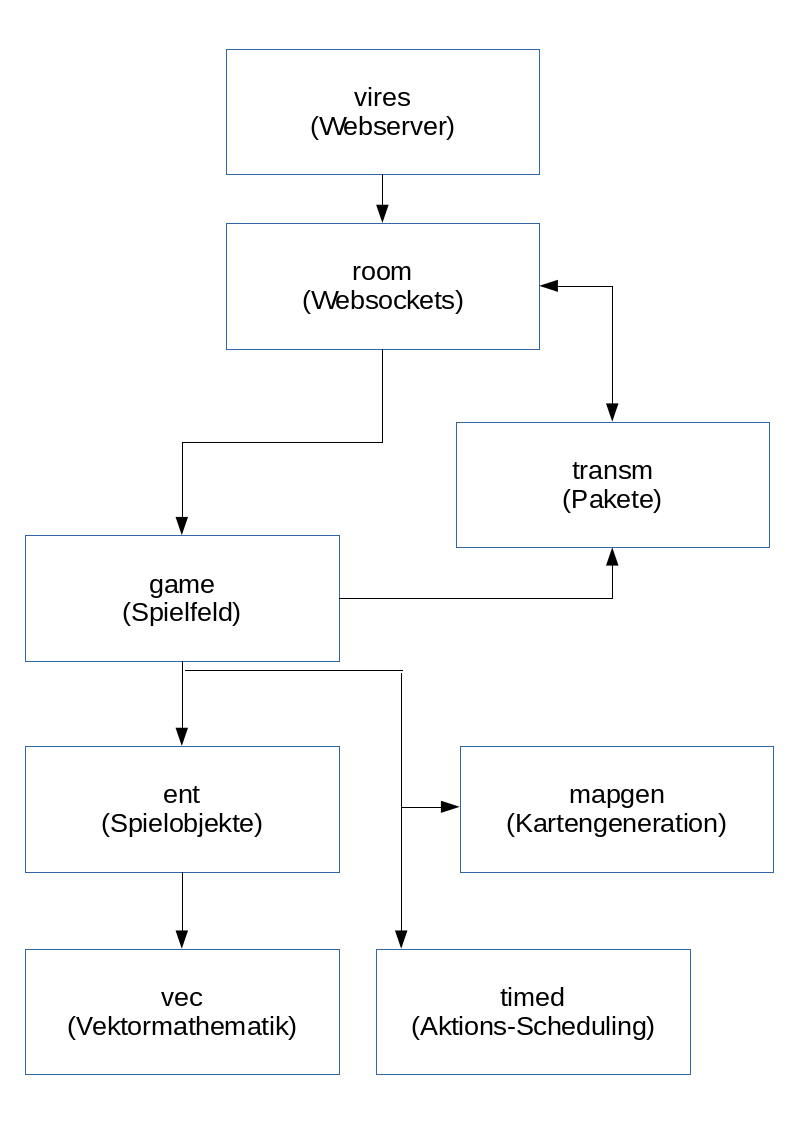
\includegraphics[width=0.6\textwidth]{Architektur.png}
	\caption{Paketaufbau des Backends}
\end{figure}
Die Bedeutung der einzelnen Pakete und wichtige Algorithmen werden im Folgenden erklärt.

\subsubsection{vires}
\verb+vires+ ist das Main-Package des Programms und kümmert sich um die Verwaltung des Webservers von \vires. \\
Wird eine GET-Anfrage auf einen Link ausgeführt, der eine Room-ID enthält (z.B. \url{http://localhost/1234}), so wird eine Template für den Raum, welche mit der Room-ID kompiliert wird, an den User gesendet. \\
Die kompilierte Template öffnet hieraufhin eine Websocket-Verbindung zu \verb+/<roomid>/c+. \\
Der Handler für \verb+/<roomid>/c+ eröffnet dann auch serverseitig die Websocket-Verbindung und übergibt die Verbindung an die jeweilige \verb+room+-Instanz.

\subsubsection{room}
\verb+room+ verwaltet die Websocket-Verbindungen eines Rooms. Verbindet sich der erste User mit dem Room, so wird der Room erstellt. \\
Alle Operationen eines Rooms werden von einer Monitor-Goroutine verwaltet, welche den Zugriff auf alle Zustände des Rooms synchronisiert. \\
Insgesamt verwaltet die Monitor-Goroutine Spielerverbindungen, Matches, Pakete von und an Nutzer und Pakete vom Spiel. \\
Genauere Informationen über Monitor-Goroutines können unter \verb+MONITOR_GOROUTINE_REF_HIER_EINFÜGEN+ gefunden werden. \\
Wird eine Websocket-Verbindung zu dem Room hinzugefügt, so werden für diese Verbindung eine Reader- und eine Writer-Goroutine gestartet. 

\subsubsection{game}
\verb+game+ verwaltet eine Spielinstanz. Eine Spielinstanz wird als Spielfeld ausgedrückt, welches sich um alle Spieloperationen kümmert, welche das gesamte Spielfeld erfordern. \\
Der \vires-Server verfolgt einen anderen Ansatz als die meisten Serverapplikationen von Spielen: 
Anstatt innerhalb eines Game-Loops zu überprüfen, ob bestimmte Bedingungen erfüllt sind,
werden alle Aktionen vorberechnet und mittels Timern und einem Scheduler verzögert, bis die Aktion ausgeführt werden soll. \\
\vires\ ist langsam und der Server soll in der Lage sein, sehr viele Matches gleichzeitig auszuführen. 
Würde der Server für jedes Match Game-Loops verwenden, so wäre entweder die Bearbeitungszeit sehr schlecht oder eine hohe
Überprüfungsfrequenz würde Serverleistung verschwenden. \\
\verb+room+ kommuniziert mit \verb+game+, indem es Methoden von \verb+game+ aufruft, wenn Nutzereingaben erfolgen. \\
\verb+game+ kommuniziert mit \verb+room+, indem es Nachrichten über \verb+transm+ nach \verb+room+ schickt, wenn das Spiel den Spielern etwas mitteilen muss. \\
Insgesamt verwaltet \verb+game+ Movements, Collisions und Conflicts. Jede Aktion auf dem Spielfeld wird über den \verb+timed+-Scheduler
ausgeführt, um Zustandszugriffe vom Spiel und von Nutzern zu synchronisieren. \\
Wird ein Movement gestartet, so wird zuerst geprüft, ob das Movement erlaubt ist. Ist es erlaubt, so wird ein Movement erzeugt, 
ein Conflict am Zeitpunkt des Conflicts für die Target-Cell geschedulet und mit jedem anderen Movement geprüft, ob es eine Collision gibt. \\
Gibt es eine Collision, so wird die Collision beiden kollidierenden Movements hinzugefügt und für den Zeitpunkt der Collision geschedulet.
Tritt der Conflict auf, so wird das Movement entfernt, die Anzahl an Moving Vires je nach Art des Conflicts der Cell hinzugefügt oder der Cell abgezogen,
überprüft, ob die Cell den Besitzer gewechselt hat, überprüft, ob der Besitzer tot ist und geprüft, ob ein Spieler das Match gewonnen hat. \\
Tritt eine Collision auf, so kämpfen die Movements miteinander oder vereinen sich je nach Art der Collision.
Hieraufhin werden alle Collisions beider Movements entfernt und neu berechnet, da die Anzahl an Moving Vires die Größe und die Geschwindigkeit beeinflusst und sich somit auch die Situation für zukünftige Collisions ändert.
Stirbt eines der Movements, so wird der Conflict für das jeweilige Movement entfernt. \\
Es wird also insgesamt beim Erzeugen eines Movements berechnet, welche Collisions nach der aktuellen Situation auftreten können, 
verändert sich aber die Situation auf dem Spielfeld, so werden erst zum Zeitpunkt der Situationsveränderung die jeweiligen Änderungen 
an den anliegenden Movements vorgenommen. \\
Beim Erzeugen der Movements wird zuerst nur davon ausgegangen, dass die auftretenden Collisions alle mit der Startgröße und der Startgeschwindigkeit stattfinden. \\
Hieraus ergibt sich, dass lediglich die anliegenden Movements verändert werden müssen, und nicht rekursiv alle Movements die nach der aktuellen Collision stattfinden. \\
Das folgende Szenario ist anzunehmen:
\begin{figure}[H]
	\centering
	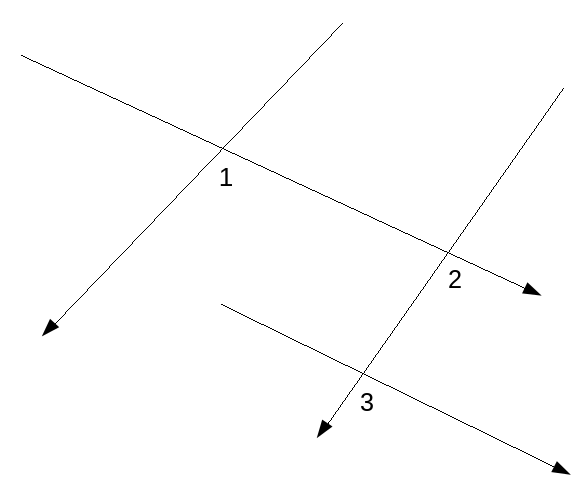
\includegraphics[width=0.8\textwidth]{Collision.png}
\end{figure}
Movements werden als Pfeile dargestellt. Alle vier Movements werden zeitnah hinzugefügt. Beim Hinzufügen aller Movements wird bestimmt, dass mit der Startgeschwindigkeit und dem Startradius des Movements die drei Collisions 1, 2 und 3 in der genannten Reihenfolge stattfinden. Für jede Collision wird für den Zeitpunkt der Collision nach Startgeschwindigkeit und Startradius eine Collision geschedulet. \\
Zuerst tritt Collision 1 auf. Hieraus ergeben sich drei Fälle für Collision 2:
\begin{enumerate}
	\item Collision 2 findet nicht mehr statt (Das Movement wurde zerstört)
	\item Collision 2 findet schneller statt (Das Movement ist kleiner geworden)
	\item Collision 2 finden langsamer statt (Das Movement hat sich mit dem anderen Movement vereint)
\end{enumerate}
In der Folge auf Collision 1 werden alle Collisions der beiden anliegenden Movements aktualisiert. \\
\begin{itemize}
	\item Tritt Fall 1 ein, so wird Collision 2 entfernt und Collision 3 findet wie erwartet mit Startgeschwindigkeit und Startradius statt
	\item Tritt Fall 2 oder 3 ein, so wird Collision 2 stattfinden, und hierbei die Geschwindigkeit und der Radius während Collision 2 angepasst
\end{itemize}
Es ist also nur nötig, die Collisions, welche mit den kollidierenden Movements verbunden sind, zu aktualisieren, da Fall 1 vom Default abgedeckt wird, während Fall 2 und Fall 3 in dem jeweiligen Zeitpunkt bestimmt werden können. Würde Fall 1 nicht vom Default abgedeckt werden, so müsste man rekursiv alle Collisions aktualisieren, die direkt und indirekt mit den betroffenen Movements verbunden sind, da die Kollisionszeit von Collision 3 aktualisiert werden müsste, und somit auch für alle damit verbundenen Movements. \\

Dieser Algorithmus verhält sich gegenüber einigen Alternativen wie folgt:
\begin{itemize}
	\item Feststellen der nächsten Collision beim Hinzufügen jedes Movements und bei jeder Collision 
	($T(\frac{n \cdot (n - 1)}{2})$, bzw. $\mathcal{O}(n^2)$, beim Hinzufügen von Movements und bei Collisions)
	\item Rekursive Erfassung der Collisions beim Hinzufügen eines Movements und beim Stattfinden einer Collision 
	($T(\frac{n \cdot (n - 1)}{2})$, bzw. $\mathcal{O}(n^2)$, beim Hinzufügen von Movements und bei Collisions)
	\item Rekursive Erfassung der kompletten Spielsituation beim Hinzufügen eines Movements 
	($T(\frac{n \cdot (n - 1)}{2})$, bzw. $\mathcal{O}(n^2)$, beim Hinzufügen eines Movements)
	\item Einfache Erfassung der anliegenden Movements bei der Collision und Annahme, dass alle Collisions unverändert stattfinden beim Hinzufügen eines Movements 
	($T(n)$, bzw.  $\mathcal{O}(n)$ beim Hinzufügen eines Movements und bei Collisions)
\end{itemize}
Die Zustandsraumkomplexität des Algorithmus ist $\mathcal{O}(n^2)$, da sich für jedes Movement bis n Movements gemerkt werden müssen.
Es wäre möglich, die Zustandsraumkomplexität weiterhin auf $\mathcal{O}(n)$ zu reduzieren, indem man sich lediglich die nächste Collision eines Movements anstatt alle Collisions eines Movements merkt, was allerdings in anderen Bereichen für größere Kosten sorgen würde und schwerer umzusetzen ist, als die aktuelle Version des Algorithmus.

\subsubsection{transm}
\verb+transm+ enthält alle Typen, welche für die Datenübertragung und die Verbindung zwischen \verb+room+ und \verb+game+ benötigt werden.
Der Transmitter in \verb+transm+ sorgt dafür, dass Typen aus \verb+game+ in Pakete umkonvertiert werden, welche dann von \verb+room+ an die Spieler weitergeleitet werden können. Immer wenn \verb+game+ den Spielern etwas mitteilen möchte, geschieht dies über \verb+transm+. \\
Alle anderen Typen in \verb+transm+ sind Typen, die ein Paket oder einen Teil eines Pakets repräsentieren, und sowohl zum Senden als auch zum Empfangen verwendet werden. Bei der Datenübertragung werden diese Typen entweder in das Übertragungsformat JSON serialisiert, oder es wird von JSON in diese Typen serialisiert. \\
\verb+transm+ enthält außerdem eine Main-Funktion, welche dazu verwendet werden kann, um ein JSON-Beispiel für das Übertragungsprotokoll zu generieren.

\subsubsection{ent}
\verb+ent+ beschäftigt sich mit den Entities auf einem Feld und kümmert sich um alle Operationen zwischen Entities, die ohne das gesamte Feld ausgeführt werden können. \\
Als solches kümmert es sich um Operationen auf den Cells, auf Movements und auf Spielern. \\
Den wohl wichtigsten und komplexesten Teil von \verb+ent+ macht die Kollisionsbestimmung zwischen zwei Movements aus. Da die \vires-Kollisionsbestimmung eine \textit{priori}-Kollisionsbestimmung ist, damit die Timer-Architektur des Spiels verfolgt werden kann, müssen Kollisionen im Vorraus mathematisch festgestellt werden. \\
Wir betrachten die Bewegung des Movements als eine Vektorgerade $g: \vec{x} = \vec{a} + t \cdot \vec{d}$. $\vec{x}$ ist die neue Position des Movements, $\vec{a}$ die Ausgangsposition des Movements, $t$ die vergangene Zeit und $\vec{d}$ der Richtungsvektor des Movements, wobei $|d| = \sqrt{{d_x}^2 + {d_y}^2}$ die Geschwindigkeit des Movements repräsentiert. Die Cells können als Kreise ausgedrückt werden. Für Kreise gilt, dass die Differenz zwischen einem Punkt auf dem Außenkreis und dem Mittelpunkt genau dem Radius entsprechen muss, es gilt also $c: r = |\vec{u} - \vec{m}|$. Betrachtet man dann den Mittelpunkt des Kreises als Gerade, so ergibt sich $r = |\vec{u} - \vec{a} - t \cdot \vec{d}|$.\\
In \vires\ kollidieren zwei Movements, wenn sich der Mittelpunkt des kleineren Movements im größeren Movement befindet, also wenn $|m_1 - m_2| < r_1$. Vereinfacht interessieren uns aber nur die Schnittpunkte des Mittelpunkts des kleineren Movements mit dem Außenkreis des größeren Movements, da das kleinere Movement nach der Collision verschwindet. Es ist also nicht wichtig, dass $|m_1 - m_2| < r_1$, da uns nicht interessiert, über welchen Zeitraum sich das kleinere Movement im größeren Movement befindet. Diese Vereinfachung ermöglicht es uns, das Problem auf folgendes zu reduzieren: Wir wollen die Schnittpunkte der Vektorgerade des kleineren Movements $g: \vec{x} = \vec{a} + t \cdot \vec{d}$ mit dem Außenkreis des größeren Movements $c: r = |\vec{u} - \vec{m}|$ bestimmen. 
Um das Problem weiter zu vereinfachen, betrachten wir die Bewegung des kleineren Movements relativ zu dem des größeren Movements, anstatt beide Bewegungen parallel zu betrachten. Hieraus ergibt sich die Gleichung $\vec{x_r} = \vec{x_1} - \vec{x_2}$, wobei $\vec{x_1}$ das größere der beiden Movements darstellt.
Insgesamt muss also diese relative Vektorgerade den Außenkreis des größeren Movements, welches sich aufgrund der relativen Betrachtung in $m(0, 0)$ befindet, schneiden. Dies ergibt $r = |\vec{x_r} - \vec{0}|$, bzw. $r = |\vec{x_r}|$. Löst man nun die Substitution auf, so ergibt sich $r = |\vec{x_1} - \vec{x_2}|$ und 
hieraufhin $r = |\vec{a_1} + t \cdot \vec{d_1} - (\vec{a_2} + t \cdot \vec{d_2})|$, bzw. $r^2 = (\vec{a_1} + t \cdot \vec{d_1} - (\vec{a_2} + t \cdot \vec{d_2}))^2$. 
Stellt man diese Gleichung mittels quadratischer Ergänzung für Skalarprodukte und Substitution für Distanzen um, so erhält man:
\begin{equation*}
\begin{split}
i_{1,2} = & \pm \sqrt{\frac{(\vec{m_1} - \vec{m_2}) \cdot (\vec{d_1} - \vec{d_2})}{|\vec{d_1} - \vec{d_2}|}^2 - (m_{1_x} - m_{2_x})^2 - (m_{1_y} - m_{2_y})^2 + (r_1 \vee r_2)^2} \\
  & - \frac{(\vec{m_1} - \vec{m_2}) \cdot (\vec{d_1} - \vec{d_2})}{|\vec{d_1} - \vec{d_2}|}
\end{split}
\end{equation*}
Mit dieser Funktion lässt sich dann berechnen, nach welchen Strecken die Collision stattfindet.
\begin{enumerate}
\item Sind $i_1$ und $i_2$ beide positiv, so findet die Collision bei der kürzesten der beiden Strecken statt: $t_c = \frac{i_1 \wedge i_2}{|\vec{d_1} - \vec{d_2}|}$
\item Sind $i_1$ und $i_2$ beide negativ, so fand die Collision in der Vergangenheit statt
\item Ist eine der beiden Strecken positiv und die andere negativ, so findet die Collision in diesem Moment statt
\end{enumerate}
Eine Visualisierung dieser Berechnung kann hier gefunden werden: \url{http://tube.geogebra.org/material/simple/id/2757139}
\subsection{Frontend}
Das Frontend besteht aus sieben Dateien, die sich in grob in fünf Bereiche unterteilen lassen.

\subsubsection{Setup} (\verb+vires.coffee+)
Dies ist der Einstiegspunkt des Codes. Hier finden die Initialisierung der anderen Programmteile, sowie alle Zugriffe auf das \verb+document+ statt. 
Nachdem die Seite fertig geladen ist, werden zunächst Callbacks für alle Maus-bezogenen Events gesetzt. Diese Callback-Funktionen setzen lediglich Flags für die entsprechenden Inputs, da sie sonst während eines Frames Daten verändern könnten, was leicht zu Fehlern führen kann.
Als nächstes wird der \verb+WebGLRenderingContext+ des \verb+<canvas>+-Elements (i.F. Viewport) initialisiert. Falls der Browser des Nutzers kein WebGL unterstützt, wird nur ein Fehler ausgegeben und das Programm beendet. Andernfalls werden danach die drei anderen Komponenten initialisiert.
Der letzte Schritt des Setups besteht darin, den Main-Loop des Spiels zu starten.

\subsubsection{Logik} (\verb+game.coffee+)
In dieser Datei ist sämtlicher Code, der direkt mit der Spiellogik zu tun hat. Sie enthält mehrere \verb+states+, welche verschiedene Zustände des Clients darstellen.
\begin{itemize}
	\item \verb+loading+ ist der Startzustand, er enthält quasi keine Funktionalität. Seine einzige Aufgabe ist es, auf den Verbindungsaufbau zu warten und währenddessen eine Animation anzuzeigen. Diese Animation dient hauptsächlich dem Zweck, zu erkennen, ob der Clent abgestürzt ist. Sobald eine WebSocket-Verbindung zum Server aufgebaut wurde, wechselt der Zustand zu \verb+lobby+
	\item \verb+lobby+ hat momentan kaum mehr Funktionalität als \verb+loading+. Auch hier wird hauptsächlich eine Animation angezeigt. Zukünftig soll es hier möglich sein, alle Spieler im Raum zu sehen, in den Zuschauer-Modus und zurück zu wechseln und das Spiel direkt zu starten. Momentan gibt es für das Beitreten anderer Spieler aber keinen Indikator und das Match muss über einen Link gestartet werden. Sobald der Client vom Server den Spielstart mitgeteilt bekommt, wechselt der Zustand zu \verb+match+.
	\item \verb+match+ ist der der komplexeste Zustand. Er ist für die Verarbeitung des eigentlichen Spiels zuständig. Dabei müssen Nutzereingaben verarbeitet, Objekte animiert und Pakete gesendet, sowie verarbeitet werden.
	Eine Reaktion auf Nutzereingaben ist das Anpassen von Position und Zoom der Kamera. Hierbei wird die Kamera so bewegt, dass es scheint, als würde der Nutzer das Spielfeld verschieben. Gleichzeitig wird aber verhindert, dass die Kamera das Spielfeld verlässt oder zu extem zoomt.
	Die zweite Reaktion auf Nutzereingaben ist das Markieren von Cells und das Senden von Movements, wobei nur Cells, die dem Nutzer gehören, markiert werden. Beendet der Nutzer seine Selektion mit dem Cursor über einer Cell, so wird dem Server der vom Nutzer durchgeführte Angriff übertragen.
	Damit Spielobjekte animiert werden, muss der Client lediglich bei jedem Tick die Position und Größe von Objekten anpassen.
	Als letztes muss der Client alle vom Server empfangenen Pakete verarbeiten und seine lokale Darstellung des Spielfeldes dementsprechend anpassen.
\end{itemize}

Damit empfangene Daten vom Client leicht verarbeitet werden können, existieren einige Klassen, die jeweils bestimmte tTile von Server-Paketen zu nutzbaren Objekten parsen. Außerdem vefügen diese Klassen über Funktionen um ihre Darstellung zu erleichtern.

\subsubsection{Verbindung} (\verb+connection.coffee+)
Diese Datei ist verantwortlich für die Client-Server-Kommunikation. Wird ein Paket vom Server empfangen, wird es hier geparsed und die resultierenden Daten werden zwischengespeichert. Diese Daten können dann im nächsten Frame von der Logik bearbeitet werden.
Soll ein Paket an den Server gesendet werden, wird umgekehrt verfahren. Zunächst werden in einem Wrapper die entsprechenden Header verpackt. Danach wird der Datensatz in einen JSON-String konvertiert und dieser wird an den Server gesendet.

\subsubsection{Grafik} (\verb+render.coffee+)
Die Grafik ist für die Kommunikation mit der Grafikkarte via WebGL und damit auch für das erzeugen des Bildes zuständig. Beim Start des Programms muss sie zunächst Speicher auf der Grafikkarte reservieren und die verschiedenen Ressourcen in den Grafikspeicher laden. Anschließend muss sie die verschiedenen Daten im Grafikspeicher verknüpfen, damit das eigentliche Rendering schnell unmd fehlerlos abläuft. Für diese Aufgaben existieren verschiedene Klassen, die zur Handhabung der unterschiedlichen Ressourcen dienen.
Während jedes Frames ist es dann lediglich nötig, eine minimale Menge von Daten und Befehlen an die Grafikkarte zu schicken, damit das gewünschte Bild entsteht.


\subsubsection{Ressourcen} (\verb+shaders.coffee+, \verb+meshes.coffee+ \& \verb+materials.coffee+)

Bei den Ressourcen handelt es sich fast ausschließlich um Daten, die, um ihr Parsing zu erleichtern, bereits in Codeform vorliegen.
Beim Initialisieren des Spieles werden die verschiedenen Ressourcen aus diesen Dateien durch das Grafikpaket verarbeitet. Dazu sind im Grafikpaket Klassen definiert, die für das Verarbeiten der Ressourcen zuständig sind.
\section{Erkenntnisgewinn}
Go hat sich als Backend-Sprache als praktisch erwiesen, da das Ökosystem und Go's Unterstützung für Goroutinen und Channels viele Dinge vereinfacht haben. \\
Die Menge an Sourcecode, welcher nötig war, um das Backend zu entwickeln, war deutlich geringer, als es beispielsweise in Java der Fall gewesen wäre, da Go deutlich weniger Verbosität aufweißt, als es in Java der Fall wäre.

Coffeescript war definitiv ein Schritt in die richtige Richtung im Gegensatz zu reinem Javascript, jedoch gibt es auch nach wie vor in Coffeescript eine Menge Fallen, in die man erst zur Runtime fällt, was die Entwicklung deutlich erschwert.

Gorilla hat sich ebenfalls als sehr nützliches Framework gezeigt. Der Grund hierfür ist hauptsächlich, dass Gorilla nicht versucht, mittels Inversion Of Control dem eigenen Code die Kontrolle zu entreißen, was bedeutet, dass für die Nutzung des Frameworks lediglich Go-Code und keine externen Tools benötigt werden. Der Lernaufwand ist also deutlich geringer - und der entstandene Code liest sich, als würde man eine Library verwenden.
Der Webserver, das Routing des Webservers und die Verwendung von Websockets haben sich deshalb als sehr einfach erwiesen.

Die Verwendung von Goroutinen und Channels hat sich in einigen Bereichen unseres Projekts als sehr nützlich erwiesen. Für die Verbindungen der User, den Scheduler und die Verbindung zwischen verschiedener Komponenten des Programms stellen Channels eine sehr gute Lösung dar. \\
Ist das Problem allerdings zustandsorientiert in seiner Natur, so ist die Verwendung von Channels nicht mehr viel praktischer als die Verwendung von Mutexes. Für ein solches Problem gibt es drei mögliche Lösungen: Entweder man verwendet ein Lock, man verwendet eine Monitor-Goroutine oder man verwendet einen Channel als Lock. Die erste Lösung ist wahrscheinlich die performanteste, da keine extra Goroutine zur Synchronisation benötigt wird, während sich bei der Verwendung einer Monitor-Goroutine alle synchronisierten Operationen an einer Stelle im Code befinden, was die Synchronisation relativ leicht überblickbar macht.

Die Timer-Architektur hat sich dagegen als nicht wirklich erfolgreich gezeigt. Da wir noch nicht in der Lage waren, den Server wirklich unter einer großen Load zu testen, können wir keine wirkliche Aussage über die wirkliche Performanz dieses Ansatzes treffen. Tests mit wenigen Rooms und fünf Spielern haben allerdings gezeigt, dass der Server ohne Probleme die Load verarbeiten konnte und zu allen Zeiten, mit Ausnahme der Generierung einer Map, bei einem Intel i5 2500k 4x3.3GHz die Prozessorauslastung des Serverprogramms <0.1\% war und der Speicherverbrauch ebenfalls lediglich bei <15MB blieb.\\
Klar ist allerdings, dass diese Architektur deutlich komplizierter zu entwickeln ist und einen stark in seiner Entwicklung einschränkt. Da alle Kollisionen im Voraus bestimmt werden müssen, muss ein Priori-Kollisionsalgorithmus verwendet werden, welcher deutlich komplizierter als die meisten Posteri-Kollisionsalgorithmen ist. Für den Priori-Kollisionsalgorithmus mussten wir unseren eigenen Algorithmus entwickeln, während wir mit einer Posteri-Kollisionsdetektion lediglich einen Quad-Tree hätten verwenden müssen. Auch das Scheduling von Timern ist nicht einfach, und besonders die mathematische Bestimmung der Kollisionszeit ist ziemlich kompliziert. Hinzu kommt noch, dass ein Priori-Kollisionsalgorithmus die Möglichkeit verhindert, geometrische Objekte zu verwenden, die nicht leicht mithilfe von Vektoren ausgedrückt werden können. Sich bewegende Kreise sind noch vergleichsweise einfach zu implementieren, während sich rotierende Dreiecke ein im Bezug auf die Performanz fast unlösbares Problem darstellen würden. \\
Trotzdem hat ein Priori-Kollisionsalgorithmus den Vorteil, dass es nicht passieren kann, dass sich Movements innerhalb eines Frames kreuzen können, ohne dass eine Kollision festgestellt wird, wenn sich die Movements zu schnell bewegen. \\
Insgesamt würden wir diese Entscheidung aufgrund ihren limitierenden Implikationen nicht erneut treffen.

Während dem Schreiben des Programms wurden verschiedene Go-Datentypen gebenchmarkt. Im Spiel gibt es überall Listen, die ungeordnet sind, bei denen aber auch trotzdem oft Lookups, Inserts und Removes erfolgen. Gebenchmarkt wurden Slices und Maps, sowie ``generische'' Versionen dieser Typen mithilfe von \verb+interface{}+ (was im Grunde \verb+Object+ in Java entspricht). \\
In der Theorie sollte die Iteration über Maps langsamer von statten gehen als bei Slices, da es bei der Iteration zu Cache-Misses kommt. \\
Das Lookup und Inserten sollte dagegen bei Slices langsamer sein. \\
Bei Removes sollten sich Slices und Maps ähnlich verhalten, da die Ordnung der Slices nicht eingehalten werden muss. \\
Zudem sollten die Versionen mit \verb+interface{}+-Typen deutlich langsamer sein als ihre konkreten Versionen, da es hierbei bei jedem Zugriff zu Cache-Misses kommt und Casts zu den konkreten Typen auch nicht unbedingt billig sind. \\

Im Folgenden sind USlices unsortierte Slices mit \verb+interface{}+, Slices sind unsortierte Slices mit einem konkreten Typen, Set sind Maps mit \verb+interface{}+ als Key und CoherentSet sind Maps mit konkreten Typen als Key. \\
Die Benchmarks haben das Folgende ergeben:
\begin{figure}[H]
\begin{tabular}{ l | c | r }
Benchmark & iterations & time/iteration \\
\hline
BenchmarkUsliceAdd & 10000000 & 149 ns/op \\
BenchmarkSetAdd	& 3000000 & 465 ns/op \\
BenchmarkSetLookup & 10000000 & 363 ns/op \\
BenchmarkUsliceLookup & 10000 & 831147 ns/op \\
BenchmarkCoherentSetLookup & 20000000 & 88.1 ns/op \\
BenchmarkSliceLookup & 200000 & 170624 ns/op \\
BenchmarkUsliceFilter & 100000000 & 144 ns/op \\
BenchmarkSetFilter & 5000000 & 322 ns/op \\
BenchmarkSliceFilter & 300000000 & 7.09 ns/op \\
BenchmarkCoherentSetFilter & 10000000 & 101 ns/op \\
BenchmarkUsliceRemove & 10000 & 511529 ns/op \\
BenchmarkSetRemove & 10000000 & 457 ns/op \\
BenchmarkSliceRemove & 200000 & 45687 ns/op \\
BenchmarkCoherentSetRemove & 20000000 & 167 ns/op \\
\hline
\end{tabular}
\end{figure}
\section{Zielreflexion}
Von den angestrebten Zielen wurde lediglich das Ziel erreicht, das eigentliche Spiel und die Map-Generation zum Laufen zu bekommen.
Hinzu kommt auch noch, dass das Frontend noch nicht so aufbereitet ist, wie es eigentlich sein könnte, was damit zusammenhängt, dass das Rendern von Text nicht mehr rechtzeitig fertig geworden ist. \\
Das Spiel selbst, wie es im Pflichtenheft beschrieben wurde, ist allerdings komplett fertig gestellt worden, mit der Ausnahme, dass das Spiel aktuell nur gewonnen wird, wenn ein Spieler der letzte Überlebende ist. \\
Die Steuerung im Frontend verhält sich ebenfalls anders, als im Pflichtenheft beschrieben, da nach mehreren Experimenten entschieden wurde, dass eine andere Steuerung intuitiver ist.

Abgesehen von den genannten Faktoren weicht die aktuelle Version von \vires\ kaum von der im Pflichtenheft beschrieben Version ab. Der komplizierteste Teil des Projekts, das eigentliche Spiel, ist abgeschlossen.
\section{Qualitätsreflexion}
\section{Projektreflexion}
Das Ergebnis des Projektes ist für uns zufriedenstellend, da wir bei der Entwicklung des Projekts eine Menge neuer Technologien angewandt und mehrere eigene Algorithmen entwickelt haben. Was den Lerneffekt angeht war dieses Projekt ein voller Erfolg - algorithmisch war dieses Projekt sehr anspruchsvoll. \\
Hiermit hängt auch zusammen, weshalb die ursprünglichen Ziele bei weitem nicht erreicht wurden: Die Komplexität vieler der zu lösenden Probleme wurde massiv unterschätzt. Das Erlernen von Go, den Konzepten von CSP, Coffeescript, Javascript, WebGL, verschiedenen Libraries, das eigene Rendern des Frontends, die Verwendung einer Timer-Architektur, die Verwendung einer Priori-Kollisionsdetektion, das Schreiben eines eigenen Schedulers und die Generation von zufälligen Maps mithilfe eines genetischen Algorithmus stellen insgesamt in der Summe eine große Aufgabe mit vielen zu lösenden Problem dar, für die es nicht immer Literatur gibt, auf die man zurückgreifen kann. \\
Die Aufgaben, welche noch nicht erfüllt wurden, weisen jedoch im Vergleich zu den erfüllten Aufgaben einen minimalen Lerneffekt auf. Insofern ist das Fehlen dieser Funktionen zwar wichtig für das Programm selbst, nicht jedoch für den Lerneffekt. \\
Das Projektmanagement des Projektes hätte deutlich besser laufen können - wäre kontinuierlich an dem Projekt gearbeitet worden, so wäre das gesamte Projekt komplett ohne Probleme fertiggestellt worden. \\
Insgesamt war das Projektmanagement mangelhaft, das Ergebnis unvollständig, die Aufgabe überfordernt - und trotzdem das Projekt ein voller Erfolg, da es viele Möglichkeiten geschaffen hat, sich mit neuen Technologien auseinanderzusetzen und komplizierte algorithmische Probleme zu lösen.
\end{flushleft}
\end{document}